\documentclass[a4paper,12pt,twoside]{book}

\usepackage{amssymb}
\usepackage{amsmath}
\usepackage{unicode-math}
\usepackage{seqsplit}

\usepackage[a4paper,top=.5in,bottom=.5in,left=.5in,right=.5in]{geometry}
\usepackage{booktabs}
\usepackage[svgnames]{xcolor}
\usepackage{pdfpages}
\usepackage{minted}
\usepackage[skins,minted]{tcolorbox}
\usepackage{csquotes}
\usepackage{fancyhdr}
\usepackage{titlesec}
\usepackage{titling}
\usepackage[hidelinks,hyperfootnotes=false,breaklinks=true,pdfauthor={Winterer, Mathis Aaron},pdftitle={Bedeutung von starken Primzahlen für die heutige Zeit},pdfsubject={Mathematische Exemplifikation des RSA-Algorithmuses},pdfkeywords={RSA,Verschlüsselung,Kryptographie,Mathematik,Primzahlen},colorlinks=true,linkcolor=black,filecolor=magenta,urlcolor=red,citecolor=blue]{hyperref}
\usepackage{tocloft}
\usepackage{fontspec}
\usepackage{polyglossia}
\usepackage[backend=biber,bibstyle=authoryear,style=alphabetic,urldate=iso,seconds=true,]{biblatex}

\setmainlanguage[variant=german,spelling=new,capitaleszett=true,babelshorthands=true]{german}
\setmainfont{IBM Plex Mono}
\setsansfont{IBM Plex Mono}
\setmonofont{IBM Plex Mono}
\setmathfont{STIX Two Math}

\graphicspath{{figs/}}
\addbibresource{bib.bib}
\definecolor{mintbg}{rgb}{0.23, 0.27, 0.29}
\definecolor{red}{HTML}{FF6961}
\usemintedstyle[csharp]{github-dark}
\setminted[csharp]{
  mathescape,
  frame=leftline,
  framesep=2mm,
  numberblanklines,
  numbersep=12pt,
  numbersep=5pt,
  baselinestretch=1.2,
  rulecolor=red,
  stripall,
  tabsize=4,
  funcnamehighlighting=true,
  autogobble,
  linenos,
  fontsize=\footnotesize,
  bgcolor=mintbg,
  breaklines,
}
\newtcblisting{cminted}[2][]{listing engine=minted, listing only,#1, title=#2, minted language=csharp, colback=mintbg}

\titleformat{\chapter}[block]{\huge\bfseries}{\thechapter.}{0.5em}{}[\titlerule\titlerule\vspace{-2em}]

\fancypagestyle{plain}{%
  \lhead{}
  \fancyhead[LO]{}
  \fancyhead[RE]{}
  \fancyhead[LE,RO]{}
  \renewcommand{\headrulewidth}{0pt}
  \fancyfoot{}
  \fancyfoot[LO]{}
  \fancyfoot[RE]{}
  \fancyfoot[LO,RE]{\thepage}
  \renewcommand{\footrulewidth}{1pt}
}

\futurelet\TMPfootrule\def\footrule{{\color{black!15}\TMPfootrule}}

\setlength{\cftsubsubsecnumwidth}{4.5em}
\renewcommand{\baselinestretch}{1.2} 
\setcounter{secnumdepth}{3}
\setcounter{tocdepth}{3}
\setlength{\parindent}{0pt}
\setlength{\footskip}{20pt}
\titlespacing*{\chapter}{0pt}{-19pt}{6em}
\renewcommand{\cfttoctitlefont}{\sffamily\bfseries\Large}
\renewcommand{\cftchapfont}{\bfseries}
\renewcommand{\cftsubsecfont}{\normalfont}
\renewcommand{\maketitle}{%
  \begin{center}
    \Huge\thetitle\\
    \vspace{1em}
    \normalsize\textit{Eine Einführung in das RSA-Verschlüsselungssystem}\\
    \vspace{2em}
    \Large\theauthor\\
    \vspace{2em}
    \large\textit{\textlang{german}{\today}}
  \end{center}
  \newpage
}

\title{Bedeutung von starken Primzahlen für die heutige Zeit}
\author{Winterer, Mathis Aaron}

\begin{document}
  \frontmatter{}
  \pagenumbering{gobble}
  \maketitle

  \pagestyle{plain}
  \pagenumbering{roman}
  \tableofcontents
  \newpage
  \listoffigures
  \newpage
  \listoftables
  \newpage

  \mainmatter{}
  \chapter{Einleitung}

Kryptographie und Verschlüsselungssysteme wurden schon im Antiken Rom verwendet um Nachrichten zu verschlüsseln\cite{aichner22}, doch heutzutage wären Verschlüsselungssysteme wie der \textquote{Cäsar-Chiffre} gegenüber eines Computers nutzlos.
Die Rolle von Kryptographie ist aufgrund des leichten Zugangs der Allgemeinheit zu leistungsstarken Computern, welche das Brechen von \textquote{schwachen} Verschlüsselungssystemen automatisiert und beschleunigt haben, um einiges angestiegen.
Aufgrund der nun verfügbaren Rechenleistung wurde die Notwendigkeit für stärkere Verschlüsselungssysteme immer größer. Zur Zeit verwendete Verschlüsselungssysteme sind so konzipiert, dass sie mathematisch schlecht rückwärts zu berechnen sind.
Hierzu werden standardmäßig große Primzahlen verwendet, da zur Zeit kein effizienter Algorithmus zur Berechnung von großen Primzahlfaktoren bekannt ist, welcher nicht die Verwendung eines Quantencomputers erfordern würde.
Das \textquote{brute-forcing} moderner Verschlüsselungssysteme ist so ineffizient, dass nur ein Teilschritt bis zu fünfzehnhundert Jahre dauern kann\cite{kleinjung10}.
\textquote{Für unsere Berechnungen waren mehr als $10^{20}$ Operationen erforderlich. Mit dem Äquivalent von fast 2000 Jahren Rechenzeit auf einem AMD Opteron mit einem Kern von 2,2 GHz [\ldots]}\cite{kleinjung10}.
Verschlüsselungssysteme sind aufgrund dieser hohen Anforderungen gegenüber der Resistenz gegen Angriffe äußerst komplexe Systeme welche in der Informationssicherheit eine entscheidende Rolle bei der Sicherung von sensiblen Daten sowohl in der Übertragung als auch bei der Speicherung spielen\cite{aichner22}.
Das Ziel dieser Facharbeit ist es den weit verbreiteten und etablierten RSA-Algorithmus zu Analysieren und zu Implementieren. Hierfür werden die einzelnen Teilschritte und verwendeten mathematischen Prinzipien und Funktionen erläutert und beispielhaft dargestellt sowie als Teil eines Programms in C\# implementiert, so dass die Funktionen der Schlüsselerzeugung, der Verschlüsselung, der Entschlüsselung und der Signierung verfügbar sind.
\newpage

\section{Hintergrund der RSA-Verschlüsselung}

$n-1=d\times{}2^j$

\begin{cminted}{MillerRabin.cs}
private static (BigInteger, BigInteger) FirstPart(BigInteger n)
{
    // nMinusOne
    BigInteger nMo = n - 1;
    BigInteger j = 0;
    BigInteger d = nMo;

    // Divide $n - 1$ By $2$ Until The Result Is Odd, Incrementing `$j$` Everytime And Storing The Result In `$d$`, So That `$n - 1 = d * 2^j$`
    while (d % 2 == 0)
    {
        d /= 2;
        j++;
    }

    return (d, j);
}
\end{cminted}
\newpage

\begin{figure}[ht]
  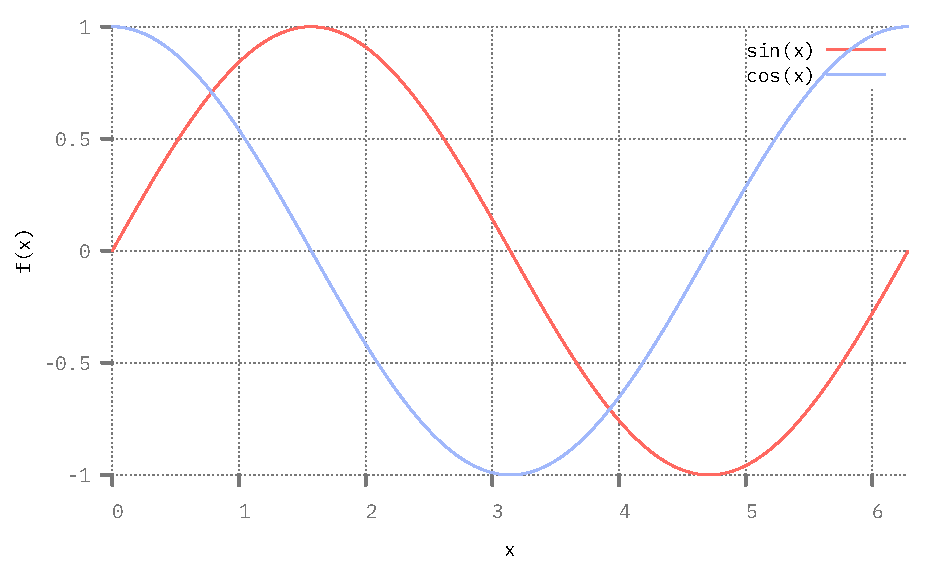
\includegraphics{sinx.pdf}
  \caption{sin(x) über [0; 6,28]}
\end{figure}

\begin{table}
  \center
\begin{tabular}{@{}llr@{}} \toprule
\multicolumn{2}{c}{Item} \\ \cmidrule(r){1-2}
Animal & Description & Price (\$)\\ \midrule
Gnat & per gram & 13.65 \\
& each & 0.01 \\
Gnu & stuffed & 92.50 \\
Emu & stuffed & 33.33 \\
Armadillo & frozen & 8.99 \\ \bottomrule
\end{tabular}
  \caption{Tabelle}
\end{table}

\newpage
\section{Anwendungsbereiche der RSA-Verschlüsselung}

  \newpage
  \chapter{Mathematische Grundlagen der RSA-Verschlüsselung}

\section{Starke Primzahlen}
\newpage
\section{Eulersche Phi-Funktion}
\newpage
\section{Carmichael-Funktion}
\newpage
\section{Euklidischer Algorithmus}
\newpage
\subsection{Erweiterter Euklidischer Algorithmus}
\newpage
\section{Hamming-Gewicht}
\newpage
\section{Chinesischer Restsatz}
\newpage
\section{Kleiner fermatscher Satz}

  \newpage
  \chapter{Anwendungsbeispiel}

\section{Schlüsselerzeugung}

Für die Erzeugung eines Schlüsselpaares werden zwei zufällige große Primzahlen $p$ und $q$ gewählt.
Um das Errechnen von $p$ und $q$ durch Faktorisierung von $n$ zu Erschweren sollten Primzahlen für $p$ und $q$ gewählt werden, welche beide \textquote{groß}\footnote{Derzeitig sichere RSA-Schlüssel besitzen zwischen $1024$-und $4096$-Bits beziehungsweise $128$-und $512$-Bytes} und \textquote{weit} auseinander liegen. Beide Primfaktoren $p$ und $q$ sind durch die Bitgröße von $n$, für welche in der Regel eine Zweierpotenz gewählt wird, beschränkt, wobei $p$ und $q$ normalerweise entweder gleich groß oder annähernd gleich groß sind. Für jeden Wert $n$ ist die Bytegröße $nB$:
\begin{align}
  \{nB \in \mathbb{N}\;|\; 6 \le nB \le 512 \}\\
  nB=\lfloor\log_2{n}\rfloor+1=\lfloor\frac{\log{n}}{\log{2}}\rfloor+1
\end{align}
So ergibt sich für $nB=512$ $p$, $q$ und $n$:
\begin{align}
\{p \in \mathbb{N}\;|\; 5 < p \le 2^{256}-1 \}\\
\{q \in \mathbb{N}\;|\; 11 < q \le 2^{256}-1 \}\\
\{n \in \mathbb{N}\;|\; 55 \le n \le 2^{512}-1 \}
\end{align}

\newpage
\section{Schlüsselverteilung}
\newpage
\section{Verschlüsselung}
\newpage
\section{Entschlüsselung}
\newpage
\section{Signatur}

  \newpage
  \backmatter{}

  \nocite{*}
  \printbibliography{}
\end{document}
